\section{Lernalgorithmen}
Die Lernalgorithmen bestimmen die Strategie, mit der die Parameter $\boldsymbol\theta$ des KNN aktualisiert werden \cite{higham2019deep}.
In dieser Arbeit wird ADAM verwendet, da dieser Algorithmus die Vorteile von \textit{(S)GD} (\textbf{S}tochastic \textbf{G}radient \textbf{D}escent)
mit Momentum und \textit{RMSprop} vereinigt \cite{kingma2014adam, higham2019deep}.
\begin{figure}[h!]
    \centering
    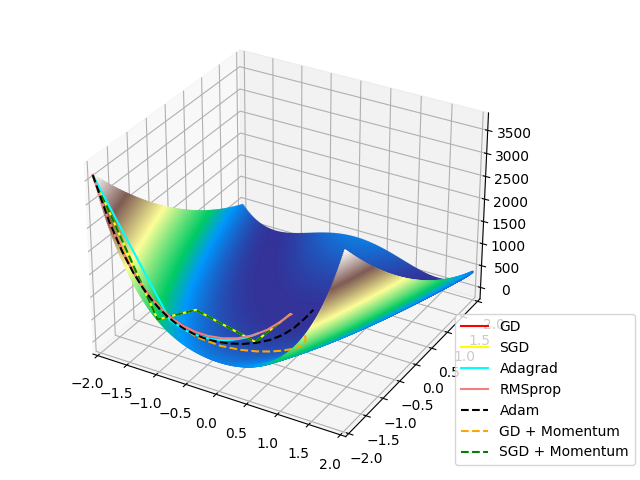
\includegraphics[width=0.8\linewidth]{images/learn_algorithms.png}
    \caption{Verschiedene Lernalgorithmen auf der Rosenbrock-Funktion \cite{rosenbrock}.}
    \label{fig:learn_algorithms}
\end{figure}
\newline
SGD ist eine Approximation von \textit{Gradient Descent} (GD) \cite{bengio2017deep}.
GD ist ein iterativer Algorithmus, der den Gradienten in Richtung des Extrema folgt und dementsprechend die Eingabeparameter aktualisiert.
\begin{align}
    \label{formular:gradient_descent}
    \theta_{k+1} := \theta_k - \text{sign}(C^{\prime}(\theta_k))\eta
\end{align}
Gleichung \ref{formular:gradient_descent} illustriert diesen iterativen Prozess für Minimierung im eindimensionalen Fall,
wobei $\eta > 0$ eine angemessene \textit{Lernrate}, $\theta$ der Eingabeparameter und $C$ die Kostenfunktion ist.
Ist die Lernrate zu groß könnte keine Verbesserung beobachtet werden, da das Maxima immer übersprungen wird.
Ist die Lernrate zu klein könnte die Konvergenz sehr langsam sein.
Wenn ein Sattelpunkt erreicht wird ist der Gradient 0.
Aus diesem Grund können mit dieser Technik globale Extrema verfehlt werden.
\newline
\newline
Im mehrdimensionalen Fall wird für jede Komponente des Eingabevektors dieser Prozess durchgeführt, sodass für jede Komponente
die Richtung des Extrema verfolgt wird.
Dies impliziert, dass GD für Eingabevektoren mit hohen Dimensionen sehr aufwendig zu berechnen ist.
Gleichung \ref{formular:gd_multi_dim} zeigt die iterative Berechnung im mehrdimensionalen Fall.
\begin{align}
    \label{formular:gd_multi_dim}
    \boldsymbol\theta_{k+1} = \boldsymbol\theta_k - \bigtriangledown C(\boldsymbol\theta_k)\eta
\end{align}
Diese Methode konvergiert, wenn alle Komponenten des Gradienten 0 sind.
Je größer die Dimension des Eingabevektor ist, desto aufwendiger ist die Berechnung.
\newline
\newline
SGD ist eine Approximation von GD. Es nutzt eine zufällige Teilmenge des Eingabevektors, den sogenannten \textit{Mini-Batch}.
Es wird angenommen, dass der Gradient des Mini-Batches ähnlich ist zu dem Gradienten des gesamten Eingabevektors.
Folglich werden mit jedem Mini-Batch die Parameter des KNN aktualisiert, wodurch in jeder Epoche die Parameter mehr als einmal aktualisiert werden.
Ziel dieser Approximierung ist eine Laufzeitverbesserung.
\newline
\newline
(S)GD mit Momentum versucht zu vermeiden, dass lokale Extrema gefunden werden anstatt globale Extrema, indem Momentum aus
vorherigen Gradienten beibehalten wird, um aus lokalen Extrema wieder raus zu finden \cite{higham2019deep}.
Gleichung \ref{formular:sgd_momentum} zeigt die iterative Berechnung.
\begin{align}
    \label{formular:sgd_momentum}
    \textbf{v}_{-1} = \textbf{0}, \hspace{0.6cm} \textbf{v}_k = \textbf{v}_{k-1}\gamma +
    \bigtriangledown C(\boldsymbol\theta_k), \hspace{0.6cm} \boldsymbol\theta_{k+1} = \boldsymbol\theta_k - \textbf{v}_k\eta
\end{align}
Zur Berechnung wird ein Hilfsvektor $\textbf{v}$ verwendet, welcher das Momentum vergangener Gradienten darstellt.
In jeder Iteration fließt ein Anteil $\gamma$, typischerweise $\gamma=0.9$, von dem Hilfsvektor in die Berechnung der neuen Eingabeparameter ein.
Der Unterschied zu GD (\ref{formular:gd_multi_dim}) ist der Anteil vergangener Gradienten.
\newline
\newline
RMSprop ist eine Generalisierung von \textit{Adagrad} \cite{mukkamala2017variants}.
Adagrad passt die Lernrate $\eta$ an, sodass Komponenten des Eingabevektors die überrepräsentiert sind eine geringere Lernrate erhalten und
unterrepräsentierte Komponenten eine im Verhältnis größere Lernrate \cite{duchi2011adaptive}.
Gleichung \ref{formular:adagrad} zeigt, wie sich iterativ die Lernrate antiproportional
zur kummulierten Norm der Gradienten der Kostenfunktion verringert \cite{lydia2019adagrad, kingma2014adam}.
Dabei wird für $\epsilon$ eine kleine Zahl gewählt, um Teilen durch 0 zu vermeiden aber keinen signifikanten Einfluss auf die Berechnung zu haben.
\begin{align}
    \label{formular:adagrad}
    \textbf{g}_k = \bigtriangledown C_{j_k}(\boldsymbol\theta_k), \hspace{0.6cm}
    \textbf{w}_k = \textbf{w}_{k-1} + \textbf{g}_k^2, \hspace{0.6cm}
    \boldsymbol\theta_{k+1} = \boldsymbol\theta_k - \textbf{g}_k \circ \frac{\eta}{\sqrt{\textbf{w}_k + \epsilon}}
\end{align}
Das Problem an Adagrad ist, dass die Lernrate zu schnell gegen 0 konvergieren kann, wodurch das Zielextrema nicht erreicht wird \cite{bengio2017deep}.
RMSprop \cite{hinton2012neural} (\ref{formular:rmsprop}) löst dieses Problem, indem anstatt die Gradienten zu summieren, ein
exponentiell gewichteter gleitender Mittelwert verwendet wird \cite{bengio2017deep}.
\begin{align}
    \label{formular:rmsprop}
    \textbf{w}_{-1} = \textbf{0}, \hspace{0.6cm}
    \textbf{g}_k = \bigtriangledown C_{j_k}(\boldsymbol\theta_k) \hspace{2.3cm} \nonumber\\
    \textbf{w}_k = \textbf{w}_{k-1}\gamma + \textbf{g}_k^2 (1-\gamma), \hspace{0.6cm}
    \boldsymbol\theta_{k+1} = \boldsymbol\theta_k - \textbf{g}_k \circ \frac{\eta}{\sqrt{\textbf{w}_k + \epsilon}}
\end{align}
Gleichung \ref{formular:adam} zeigt, wie Adam RMSprop und (S)GD mit Momentum vereint, wobei $\gamma_1 < \gamma_2 < 1$ \cite{kingma2014adam} ist.
Adam beinhaltet RMSprop und hat eine Momentum Komponente, indem der Moment der ersten Ordnung mit exponentieller Gewichtung approximiert wird \cite{bengio2017deep}.
Zudem korrigiert Adam den Bias der Momente der ersten und zweiten Ordnung der durch die Initialisierung entsteht.
\begin{align}
    \label{formular:adam}
    \textbf{v}_{-1} = \textbf{w}_{-1} = \textbf{0}, \hspace{0.6cm}
    \textbf{g}_k = \bigtriangledown C_{j_k}(\boldsymbol\theta_k) \hspace{0.4cm} \nonumber\\
    \textbf{v}_k = (\textbf{v}_{k-1}\gamma_1 + \textbf{g}_k (1-\gamma_1))/(1 - \gamma_1^k) \hspace{0.15cm} \nonumber\\
    \textbf{w}_k = (\textbf{w}_{k-1}\gamma_2 + \textbf{g}_k^2 (1-\gamma_2))/(1 - \gamma_2^k) \nonumber\\
    \boldsymbol\theta_{k+1} = \boldsymbol\theta_k - \textbf{v}_k \circ \frac{\eta}{\sqrt{\textbf{w}_k + \epsilon}} \hspace{1.1cm}
\end{align}